% !TeX root = ../defense.tex

\section{Results Update}
\frame{\sectionpage}

\begin{frame}{Motivation}
    \begin{alertblock}{How is the analytical solution computed for Sound Prop. in Uniform Axial Flow}
    \begin{enumerate}[<+->]\itemsep9pt
        \item The analytical solution are the axial wavenumbers and propagating
            modes for a given frequency, axial velocity and azimuthal mode order.
        \item For a given azimuthal mode, there is a range of radial modes.
        \item These radial modes can be categorized based on the sign of the axial wavenumber and if it is
            complex in value. 
        \item Propagating modes are defined by axial wavenumbers, $k_x$, that have a real-part only, yielding 
            the assumed fluctuation to resemble Euler's Formula ($e^{ik_x x}$). 
        \item On the other hand, if the $k_x$ is complex, then the mode will resemble an exponentially decaying
            function since the imaginary number cancels, leaving a minus sign in front of
            the axial wavenumber.
    \end{enumerate}
    \end{alertblock}

    \tiny
    % \hspace{3.75em}\url{http://www.klimaschutzplan2050.de/en/action-areas/energy-sector/}
\end{frame}
\begin{frame}

\begin{equation}
    k_x  = \frac{- M_x k \pm \sqrt{k^2 - ( 1 - M_x^2) J_{m,n}'^2 }}{\left( 1 - M_x^2 \right)}.
    \label{eqn:ax_wavenumb}
\end{equation}

where $M_x$ is the axial Mach number, $k$ is the temporal (referred to as reduced)
frequency, and $J_{m,n}'$ is the derivative of the Bessel function of the first kind.  
The $\pm$ accounts for both upstream and downstream modes.

The condition for propagation is such that the axial wavenumber is larger than 
a ``cut-off'' value

\begin{equation}
    k_{x,real}  = \frac{\pm M_x k }{\left( M_x^2 - 1 \right)}.
    \label{eqn:cuton}
\end{equation}


\end{frame}
\begin{frame}
    
Every term that is being raised to the one half i.e. square rooted must 
be larger than zero to keep axial wavenumber from being imaginary. The mode 
will propagate or decay based on this condition. Recall thaT the mode is of the 
form 
\begin{equation}
    e^{i k_x x}
    \label{eqn:fluctuationexample}
\end{equation}
if $k_x$ has a real part, $k_{x,real}$ and an imaginary part $i k_{x,imag}$ 
then,

\begin{align}
    &= e^{i k_x x} \\
    &= e^{i (k_{x,real}+ i k_{x,imag}) x} \\
    &= \underbrace{e^{i k_{x,real}x}}_{\textit{amplitude}} \underbrace{e^{- k_{x,imag} x}}_{\textit{exponential decay}} 
\end{align}


\end{frame}
\begin{frame}
    

Although the ``cut-off'' decay to nearly zero rapidly, the rate at which this occured
was not much of a concern earlier on in turbomachinery design. As nacelles 
continue to grow shorter, a mode that is ``cut-off'' may make it outside the duct.

For this work a desired amplitude was arbitrarily chosen for a mode, $y_{desired}$
and then the axial location at which this occurred, $x_{desired}$ which 
can be compared against a desired length for a nacelle.  
Since SWIRL assumes an infinitely long duct, there is nothing limiting the 
modes propagation with respect to nacelle length. For example, if the 
desired amplitude is one percent, then $x_{desired}$,

\begin{align*}
    0.01 &=  e^{-10 x_{desired}},\\
    -\frac{ln|0.01|}{10} &=  x_{desired},\\
    -\frac{ln|0.01|}{10} &= 0.4605170185988091 .
\end{align*}

\end{frame}
\begin{frame}
    


 \begin{figure}
     \centering
     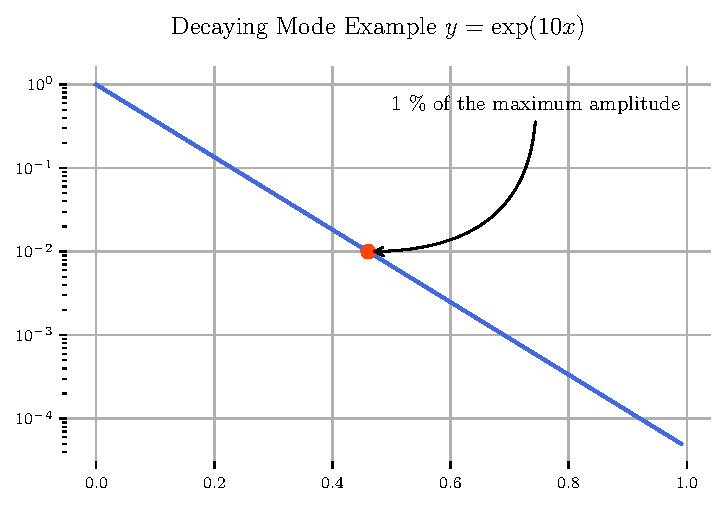
\includegraphics[width=0.7\textwidth]{/home/jeff-severino/SWIRL/CodeRun/04-plotReport/tex-outputs/desired_cut_off_location_1_percent_of_max2.pdf}
     \caption{Decaying mode with $k_x = 0 + 10j$ and unit amplitude. One percent
     of the maximum amplitude is identified for nacelle length comparison}
     \label{fig:decaying_mode_with_1_percent_amp}
 \end{figure}
 
 
In general,
\begin{align*}
    y_{desired} &=  e^{-k_{x,imag} x_{desired} }\\
    -\frac{ln|y_{desired}|}{k_{x,imag}} &=  x_{desired}
\end{align*}
\end{frame}
\begin{frame}
\section{Analytical Test Case 1}
\begin{table}[h!]
    \centering
    \begin{tabular}{|l|l|}
        \hline
        $\sigma$ & \textit{0.0} \\ \hline
        $k$      & \textit{10}   \\ \hline
        $m$      & \textit{2}    \\ \hline
        $M_x$    & \textit{0.3}  \\ \hline
    \end{tabular}
    \caption{Validation test case parameters, Uniform Flow Annular Duct} 
\end{table}

\end{frame}

\begin{frame}
    
 \begin{figure}
     \centering
     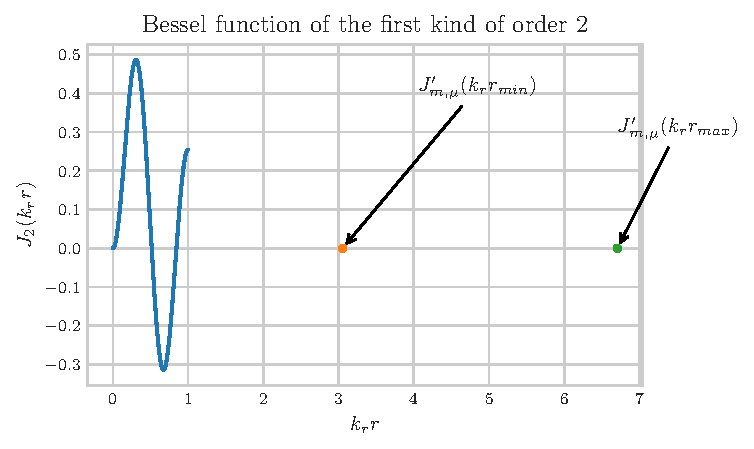
\includegraphics[width=0.7\textwidth]{/home/jeff-severino/SWIRL/CodeRun/04-plotReport/tex-outputs/bessel_analytical_test_case.pdf}
     \caption{The Bessel function with the values of $J'_{m,\mu}$ labeled}
     \label{fig:decaying_mode_with_1_percent_amp}
 \end{figure}
\end{frame}



\begin{frame}
    
 \begin{figure}
     \centering
     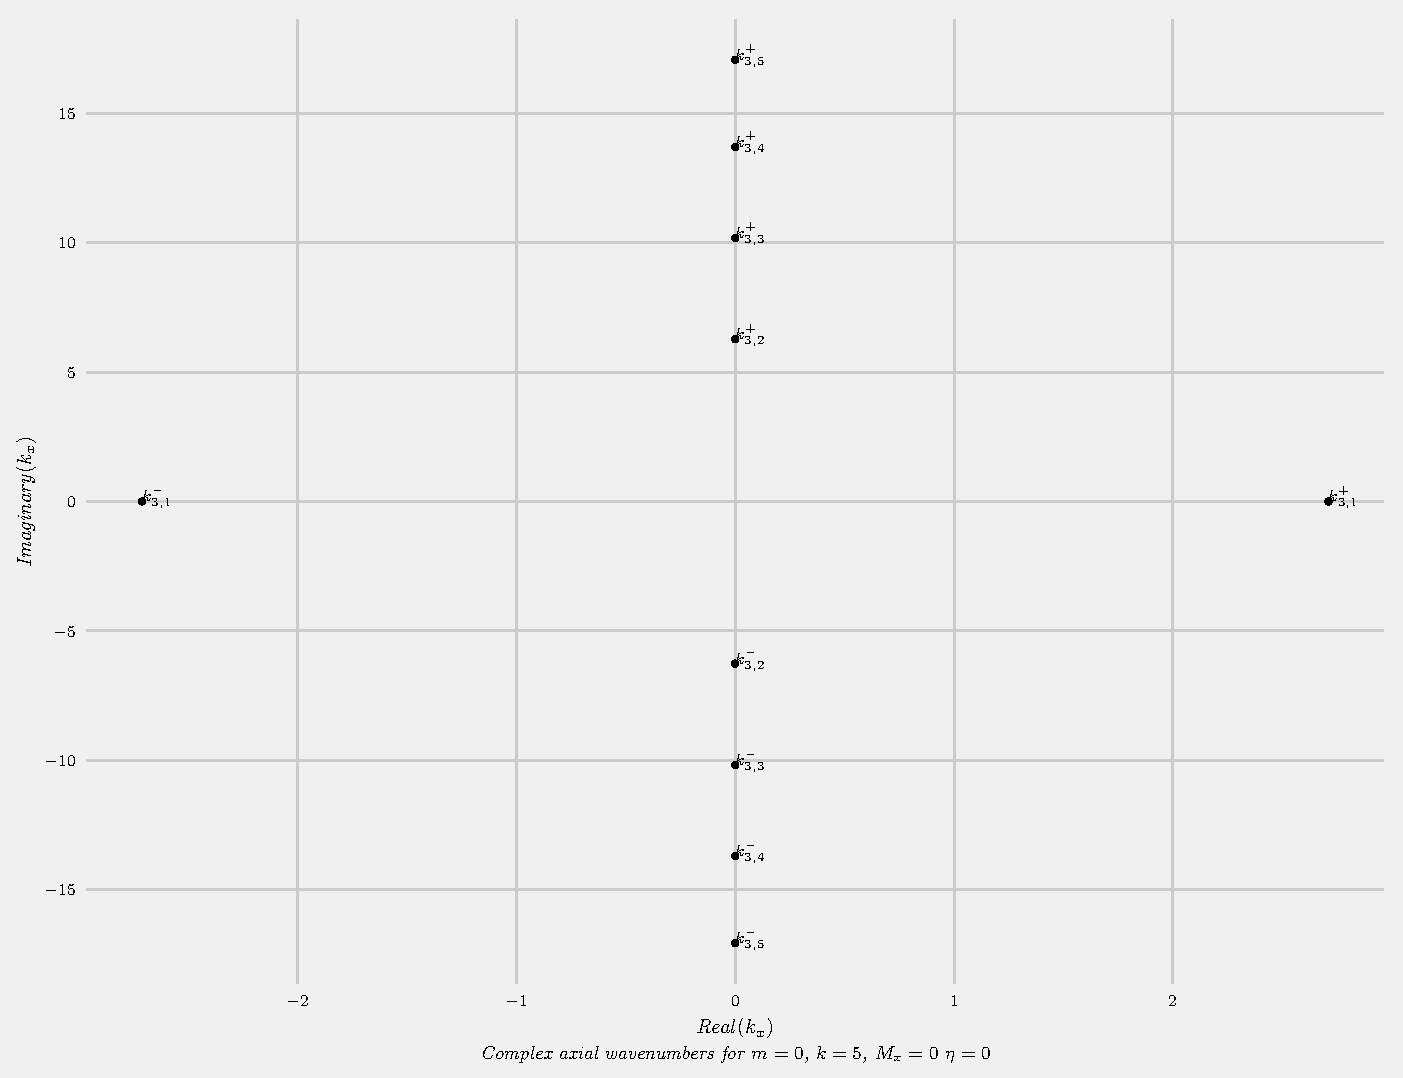
\includegraphics[width=0.7\textwidth]{/home/jeff-severino/SWIRL/CodeRun/04-plotReport/tex-outputs/axial_wavenumber_analytical_test_case.pdf}
     \caption{The Bessel function with the values of $J'_{m,\mu}$ labeled}
     \label{fig:decaying_mode_with_1_percent_amp}
 \end{figure}
\end{frame}


\begin{frame}{Normalized Mode}

    
 \begin{figure}
     \centering
     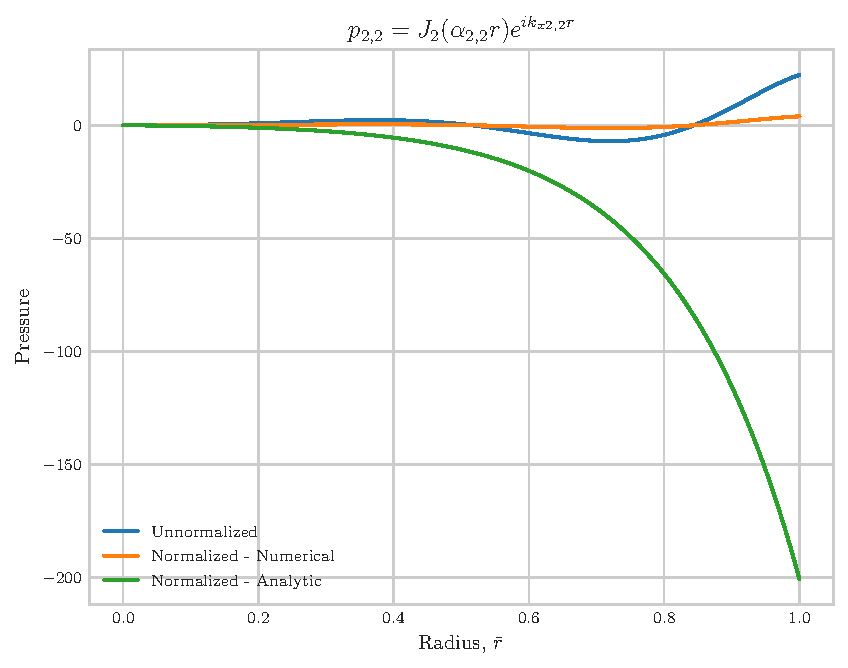
\includegraphics[width=0.7\textwidth]{/home/jeff-severino/SWIRL/CodeRun/04-plotReport/tex-outputs/Normalized_Mode_test_case.pdf}
     \caption{The Bessel function with the values of $J'_{m,\mu}$ labeled}
     \label{fig:decaying_mode_with_1_percent_amp}
 \end{figure}
\end{frame}
\begin{frame}
    
\end{frame}




\begin{frame}{Future Work}
    \begin{alertblock}{}
    \begin{enumerate}[<+->]\itemsep9pt
        \item I need to use sanity checks to ensure that the normalization provided
            by Rienstra is implemented correctly.
        \item While the numerical normalized mode has an integral of one, the 
            analytical mode is not.
        \item a few things that have been checked along the way but need to be 
            reported are,
        \item Zero's of $J'_m$ 
        \item Value of $J_m$ at the zero location
        \item Relations involving integrals If it so not too cumbersome.
            There are some simplifications that could be checked\ldots 
        \item Check the analytical test case that has been reported in literature.
           The difference is that $\sigma = 0.25$
    \end{enumerate}
    \end{alertblock}

    \tiny
    % \hspace{3.75em}\url{http://www.klimaschutzplan2050.de/en/action-areas/energy-sector/}
\end{frame}

% \begin{frame}{Perspective}{Disciplines for investigating energy topics}
%     \begin{center}
%     \begin{tikzpicture}[
%       node distance=4.5em and .75cm,font=\small
%     ]
%     % flowboxes
%     \node[flowbox] (physik) {
%         \fbtitle{Physics}\vphantom{yÖ}
%     \nodepart{two}
%         \begin{minipage}{.16\textwidth}
%             \centering
%             Theoretical\\ feasibility\\
%             \scriptsize (Natural laws)
%         \end{minipage}
%     };

%     \node[flowbox,right=of physik] (technik) {
%         \fbtitle{Engineering}\vphantom{yÖ}
%     \nodepart{two}
%         \begin{minipage}{.16\textwidth}
%             \centering
%             Technical\\ feasibility\\
%             \scriptsize (Technologies)
%         \end{minipage}
%     };

%     \node[flowbox,right=of technik] (econ) {
%         \fbtitle{Economy}\vphantom{yÖ}
%     \nodepart{two}
%         \begin{minipage}{.16\textwidth}
%             \centering
%             Economic\\ feasibility\\
%             \scriptsize (Funding)
%         \end{minipage}
%     };

%     \node[flowbox,right=of econ] (society) {
%         \fbtitle{Society}\vphantom{yÖ}
%     \nodepart{two}
%         \begin{minipage}{.16\textwidth}
%             \centering
%             Social\\ feasibility\\
%             \scriptsize (Decision space)
%         \end{minipage}
%     };

%     \uncover<2->{%
%         \draw [decorate,decoration={brace,amplitude=10pt,mirror},ultra thick,jdblue]
%             ($(technik.south west) + (-.2em,-1em)$) --
%             ($(econ.south east)    + (+.2em,-1em)$) coordinate[midway,yshift=-3.8em] (midpoint-below);
    
%         \node[flowbox] at (midpoint-below) (tech-econ)  {
%             \fbtitle{Techno-economic modelling}\vphantom{yÖ}
%         \nodepart{two}
%             \begin{minipage}{.4\textwidth}
%                 \centering
%                 How much energy?
%                 For how much?\vphantom{yÖ}
%             \end{minipage}
%         };
%     }
%     \end{tikzpicture}
%     \end{center}
% \end{frame}
